\documentclass[journal,twocolumn,12pt]{ieeesyscoin}
\usepackage{cite}
\usepackage{amsmath,amssymb,amsfonts}
\usepackage{algorithmic}
\usepackage{enumitem}
\usepackage{caption}
\usepackage{xcolor}
\usepackage{graphicx}
\usepackage{textcomp}
\usepackage{multirow}
\usepackage{lipsum}
\usepackage[switch]{lineno}
\def\BibTeX{{\rm B\kern-.05em{\sc i\kern-.025em b}\kern-.08em
    T\kern-.1667em\lower.7ex\hbox{E}\kern-.125emX}}
\begin{document}
\linenumbers
\history{}

\title{\centering DAOSYS: An Autonomous Service Engine for Decentralized Finance}
\author{\centering  \uppercase{Cyotee Doge}\authorrefmark{1}, 
\uppercase{Ian C. Moore, PhD}\authorrefmark{2},
\uppercase{Ryland Arbour}\authorrefmark{3}, and
\uppercase{Jagdeep Sidhu, MSc}\authorrefmark{4}}

\address[1]{\centering DAO Advisor, Syscoin Platform (e-mail: cyotee@syscoin.org)}
\address[2]{\centering  Syscoin Researcher, Syscoin Platform (e-mail: imoore@syscoin.org)}
\address[3]{\centering  L2 Advisor, Syscoin Platform (e-mail: rylandarbour@syscoin.com)}
\address[4]{\centering Syscoin Lead Developer, (e-mail: sidhujag@syscoin.org)}
\tfootnote{}

\markboth
{Cyotee \headeretal: DAOSYS: An Autonomous Service Engine for Decentralized Finance}
{Cyotee \headeretal: DAOSYS: An Autonomous Service Engine for Decentralized Finance}

\corresp{}

\begin{abstract}
Despite popular perception, treasuries of Dentralized Autonomous Organizations (DAOs) tend to be centrally controlled and do not reflect the true ethos of cryptocurrency (i.e., \textit{not your keys, not your coins}). DAOSYS solves this problem with its new Autonomous Service Engine (ASE) technology by deploying a reference platform for self-sovereign capital coordination. This is made possible by innovating on the multi-faceted proxy standard defined in EIP-2535. The ASE will serve as the cornerstone of all SYS Labs decentralized finance (DeFi) products, as supported by the Syscoin Platform.
\end{abstract}

\begin{keywords}
DAOSYS, Decentralized Autonomous Organization, Decentralized Finance, SYS Labs, EIP-2535
\end{keywords}

\titlepgskip=-15pt

\maketitle

\section{Introduction}
\label{sec:introduction}

The objective of a decentralized autonomous organization (DAO) is to solve the principal-agent dilemma. This dilemma is a result of misaligned incentives where agents acting in a system are incentivized towards their own benefit over the benefit of a principle or other agents acting within the system \cite{San83}. Typically, these are found in centralized systems where the central acting authority is the main compromised agent. The DAO solves this by decentralizing the governance process by utilizing smart contracts running on open source blockchains.

The first inception of the DAO concept happened in May 2016 out of the Ethereum community, which was known as Genesis DAO, and was built as a smart contract on the Ethereum blockchain. However, this resulted in the well known DAO Hack which resulted in the draining of \$60M USD worth of funds from its treasury \cite{Sie22}. Today, there are many DAOs in operation with Uniswap, Aave and Maker DAO being amongst the most popular. However, these DAOs still fundamentally violate the core value proposition of self sovereignty that crypto currency promises, where DAOs currently take ownership of capital managed in a treasury controlled by a few individuals. This is the problem that DAOSYS intends to address.

DAOSYS vision is to operate like a pure automated market maker (AMM) and be implemented in a manner that does not require external controls. In 2018, Uniswap became the first decentralized platform to successfully utilize an AMM \cite{Uni19}. However, like Uniswap and many AMMs, control of the capital in their respective liquidity pools is still centralized. DAOSYS intends to address this core issue via its new Autonomous Service Engine (ASE) technology \cite{Sys22}, hence allowing DAOs to be more autonomous and fully decentralized. One of the interesting by-products of this technology will allow users to test, implement and realize countless decentralized finance (DeFi) usecase designs through the ASE without having to continually redeploy new builds.

\section{Governance}
\label{sec:governance}

DOAs are governance structures for groups of people to come together and make decisions, which is one of its main distinguishing features. Unlike traditional organizations (e.g., private companies, non-governmental organizations, charities, etc.) which have a centralized structure, these decisions are coordinated and enforced on a blockchain in a decentralized manner. Since DAOSYS proposes to be autonomous and fully decentralized, it has no top level governance.

AMMs are an essential part of the DeFi ecosystem. They allow digital assets to be traded in a permissionless and automatic way by using liquidity pools rather than a traditional market of buyers and sellers. Applying the AMM model to DAOs means that users create their own treasuries for specific ventures. These treasuries may apply a variety of governance solutions along with their treasuries. This allows for a compartmentalization of the politics that arise with any governance solution from the actual treasury management.

Under this model, the Syscoin Foundation behaves more like the software vendor. The factory makes open-source reference implementations of DeFi components available to compose into treasuries. Updates to these smart-contracts are available for deploying new pools that may be added to a DAO. Hence, this removes the need for top-level governance solutions that decides whether to include an update because users are free to create new pools.

A user creates a DAO by selecting which vaults and bond markets they would like to include. These vaults may come from one of four sources.

\subsection{Reuse an existing vault}

This works best for when users wish to maintain their position in one DAO, but want to add more pools to form a new DAO.

\subsection{Recreate an existing vault}

As the adage goes,\textit{if it’s not broke, don’t fix it}. The investment strategy implemented in a vault can be used across several instances of vault pools. This works well for new DAOs that wish to replicate the financial strategies of an existing DAO. Also, for when a new DAO would like to invest in other DAOs using the same strategy.

\subsection{New pool with new investment strategy}

A user may wish to create a new DAO reusing functionality available from the factory, but configured in a novel manner. The flexibility available in the ASE means that even a simple strategy has several configuration options. This is useful for when a DAO wishes to adopt a novel investment strategy that might not have been previously viable.

\subsection{New pool with custom code}

The Syscoin Foundation makes internal decisions regarding what smart-contracts are available through the factory similar to open source software development. Because this only concerns the software available from the foundation, this does not need to be open to public governance. When the community at large wishes to release custom code outside the foundation, a user may use the factory to deploy their own factory offering their custom code. This new factory inherits the offerings of the parent factory and may add their own modules.

These pools form the foundation of the DAO. Autonomous and permissionless liquidity pools that act as the agreed upon foundation for DAO treasury management. From there users may launch further liquidity pools that may accept the DAOs Treasury Token for deposit. These form the Roundtables for managing ventures within the DAO. The Roundtables compartmentalize management teams, Councilors, of the various ventures being executed under a DAO’s mission statement. A Roundtable typically does not have it’s own governance token, instead using a Council Token used to resolve disputes by executing buyout options.

From the Roundtables, any Councilor may use their contribution to the Roundtable to launch a bond offering for a Quest. Quests define the bounty award and terms for completing a task. The Councilor that issues the quest puts their share of the treasury in escrow to fund the Quest. The interest being earned from that underlying position is then split to fund the bounty, compound into that position, and to sell on the bond market. This ensures that Questors know the payment for work they deliver is secured. And protects the Councilor from failure to deliver; see Fig. \ref{fig:daosys_governance} for outline.

\begin{figure}[h!]
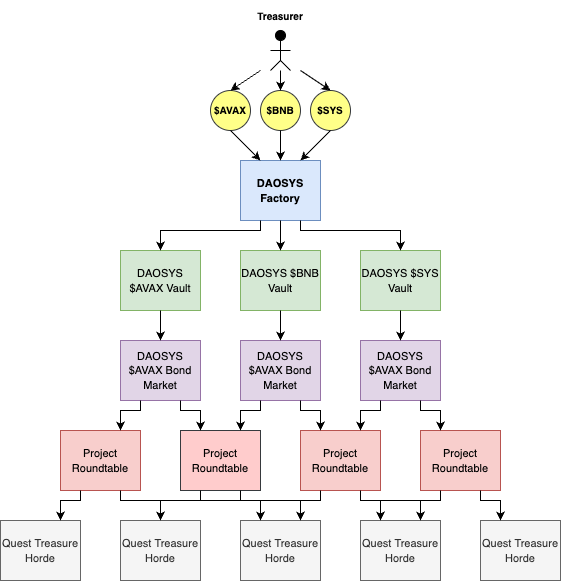
\includegraphics[width=3in]{img/governance.png}
\caption{DAOSYS Governance Structure: new pool with custom code (ie, Quests)} 
\label{fig:daosys_governance}
\end{figure} 

\section{Architecture}
\label{sec:architecture}

The innovative software architecture that allows DAOSYS to pioneer a revolution in DAOs is the ASE. This introduces a revolution allowing DAOs to become more autonomous and fully decentralized. The ASE iterates on the Diamond proxy standard from EIP-2535 (see Appendix \ref{sec:diamond}) to apply AMM functionality for more flexible capabilities.

\subsection{ICreate2Metadata}

The \texttt{CREATE2} opcode is a low level human readable instruction used within the stack-based architecture of the Ethereum Virtual Machine (EVM) that was introduced in 2019 with EIP-1014 \cite{But18}. This is the technology that enables AMMs in EVM implementations which allows a smart-contract to deploy another smart contract, and is typically called the Factory design pattern. Protocols like Balancer and Uniswap provide the ability to create permissionless liquidity pools. However, the limit of these implementations is the immutable nature of smart-contract bytecode as they can only deploy a single type of contract. 

All contracts deployed through the ASE, new service proxies and delegate service, store the metadata for their deployment. This includes the factory address they were deployed from, and the value used to salt their deployment. Combined with the contract’s \texttt{codehash} this can be used to recalculate the contract’s address from the assertion of it’s \texttt{ICreate2Metadata} interface hook.

\subsection{IDelegateService}

Protocols like Aavegotchi have pioneered smart-contract architecture by iterating on the proxy capabilities of the EVM to advance the Factory design pattern. Smart-contract proxies take advantage of the \texttt{DELEGATECALL} opcode to allow a smart-contract to reuse the logic implemented in other smart-contracts. The Autonomous Service Engine advances this innovation with an infinitely flexible Diamond Factory design. The Diamond Factory design factory combines the Factory and Diamond design patterns to deploy configurable proxies. This allows for infinitely composable proxies.

Delegate Services replace the Facets defined in ERC-2535. Delegate Services define a strict storage allocation and access standard beyond the theory presented in ERC-2535. A Service is a smart-contract or library implemented following the Deterministically Dynamic Storage Allocation standard. A Service also reports the factory that deployed that contract and the salt used during deployment. This way the recalculation of the address from the factory init code hash and salt can be used to verify new Services as an implicit ACL.

This means that the deployment process for new Services deviates from industry standard. New Services are deployed as compiled bytecode passed to the Service Proxy Factory as the argument for the deployment function. The Service Proxy Factory then instantiates that bytecode as a new contract. ASE compliant Services must include the ASEServiceBootstrapper library to retrieve the address salt to initialize the Service. This should be done by delegating to the canonical external library deployment. ASE compliant external libraries may precalculate their address salt and store it as a constant. The standard Service initialization functions must still be implemented, but may hard code the values and return values since they can not store state.

All Services are required to implement ERC-165 including the Service extension that enumerates the functions. The Service extension to ERC-165 includes a per interface enumeration of the function selectors that define the interface ID. Additionally, there is an enumeration of all the function selectors across all interface IDs, and a ServiceDef struct that includes the information for initializing a Service Proxy to consume the Service.

\section{Tokenomics}
\label{sec:tokenomics}

\lipsum[1]

\subsection{Simulator}

\lipsum[2-4]

\section{RoadMap}
\label{sec:roadmap}

\subsection{SYSLabs}

\lipsum[1]

\subsection{L2: NEVM}

\lipsum[1]

\subsection{First Use Case: Masternode Yield Farming}

\lipsum[1]

\section{Summary}
\label{section:summary}
\lipsum[1]

\appendices

\section{EIP-2535 (Diamond Facets)}
\label{sec:diamond}

EIP-2535 was an Ethereum proposal launched in 2020 to allow for the creation of modular contract systems that can be extended after deployment \cite{Mud20}. To solve this problem, this new proposal introduced a concept known as Diamonds. A Diamond refers to a smart contract system where functionality and storage is split up into separate contracts, and is an extension of a proxy contract.

A proxy contract is the the immutable part a user interacts with which holds data. It contains a fallback function which will catch any function call and use \texttt{delegatecall} to forward it to a second logic contract. As a reminder, \texttt{delegatecall} will execute a function defined in the called contract (logic), but within the context of the calling contract (proxy). Thus, we have our logic defined separately from our data. This allows users to change the logic contract without changing the immutable underlying data. 

There are several limitations to proxy contracts which include: (a) implementing minor upgrades; (b) 24kb max contract size limit; (c) can only create identical proxy instances using one logic contract; and (d) cannot have a modular permission system. Diamonds solve these issues by allowing for multiple logic contracts which talks to the original proxy contract via the \texttt{delegatecall}; for comparison between these two systems see Fig. \ref{fig:diamonds} .

\begin{figure}[h!]
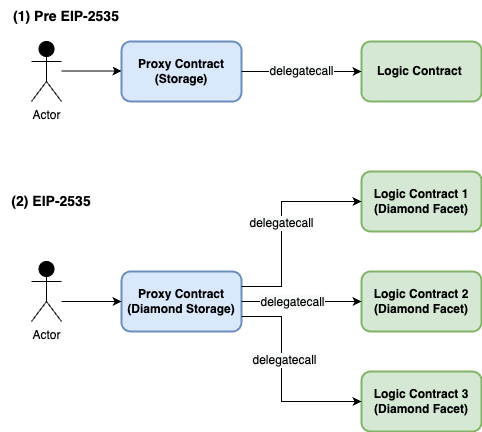
\includegraphics[width=3in]{img/diamonds.png}
\caption{Multi-facet proxy; (TOP) prior to EIP-2535, proxy contracts could only make delegates calls to another contract only; (BOTTOM) EIP-2535 introduced the capability of performing delegates calls to multiple contracts} 
\label{fig:diamonds}
\end{figure} 

\begin{thebibliography}{00}

\bibitem{San83} S.J. Grossman, O.D. Hart, \textit{An Analysis of the Principal-Agent Problem}, Econometrica, Volume 51, Issue 1 (Jan., 1983), 7-46.

\bibitem{Sie22} D. Siegel, \textit{Understanding The DAO Attack}, Coindesk, Aug. 2022. Accessed on: Sept 2022. [Online]. Available: https://www.coindesk.com/learn/2016/06/25/understanding-the-dao-attack/

\bibitem{Sys22} Syscoin Dev Team, \textit{DAOSYS Lite Paper}, Accessed on: Sept 2022.  [Online]. Available:  https://github.com/syscoin/daosys

\bibitem{Uni19} Uniswap Blog, \textit{A short history of Uniswap}, Sept. 2019. Accessed on: Sept 2022.  [Online]. Available:  https://uniswap.org/blog/uniswap-history

\bibitem{Mud20} N. Mudge, \textit{EIP-2535: Diamonds, Multi-Facet Proxy}, Aug. 2020. Accessed on: Sept 2022.  [Online]. Available: https://eips.ethereum.org/EIPS/eip-2535

\bibitem{But18} V. Buterin, \textit{EIP-1014: Skinny CREATE2}, Apr. 2018. Accessed on: Sept 2022.  [Online]. Available: https://eips.ethereum.org/EIPS/eip-1014



\bibitem{Sig21} J. Sidhu and I.C. Moore, \textit{Syscoin 4.0: A Peer-to-Peer Electronic Cash System Built For Business Applications}, Dec 2021, Accessed on: Sep 2022.  [Online]. Available:  https://syscoin.org/file/syscoin4-whitepaper.pdf

\end{thebibliography}


\EOD

\end{document}
